\documentclass[12pt, letterpaper]{article}
\usepackage{graphicx} %Latex package to import graphics (i.e. images)
\usepackage{forest} %Latex package to draw tree diagram
\usepackage{subfigure} %Latex package to provide support for small figures
\graphicspath{{etc}}
\title{Why is $ \frac{\partial J(W)}{\partial W_{i,j}^{(out)}} = (A^{(h)})^{T} \delta^{(out)}$ ?}
\author{Kassi Bertrand}
\date{January 2023}

\begin{document}
\maketitle

\section{Introduction}
In this \LaTeX{} document, I want to show my step-by-step process
to derive the partial derivative of all the weights in $W^{(out)}$.

\vspace{5mm} %5mm vertical space

I'll start simple with a 2-2-2 MLP, which is a Multi-Layer Perceptron
with 2 inputs, 2 hidden units, and 2 outputs, and then generalize
what we learn to a general $m-d-t$ MLP.

\vspace{5mm} %5mm vertical space

In both cases, I will use the following loss/error function:
\[J(w) = -\sum\nolimits_{i = 1}^{n}\sum\nolimits_{j=1}^{t} y_j^{[i]} ln(a_j^{[i]}) + (1 - y_j^{[i]})ln(1 - a_j^{[i]})\]

Where the superscript $[i]$ is an index for training examples,
and $j$ is the number of output units.

\vspace{5mm} %5mm vertical space

Ready? Let's go!

\pagebreak
\section{With a 2-2-2 MLP}

For this example, we will consider the following Neural network:

%2-2-2 MLP picture
\begin{center}
    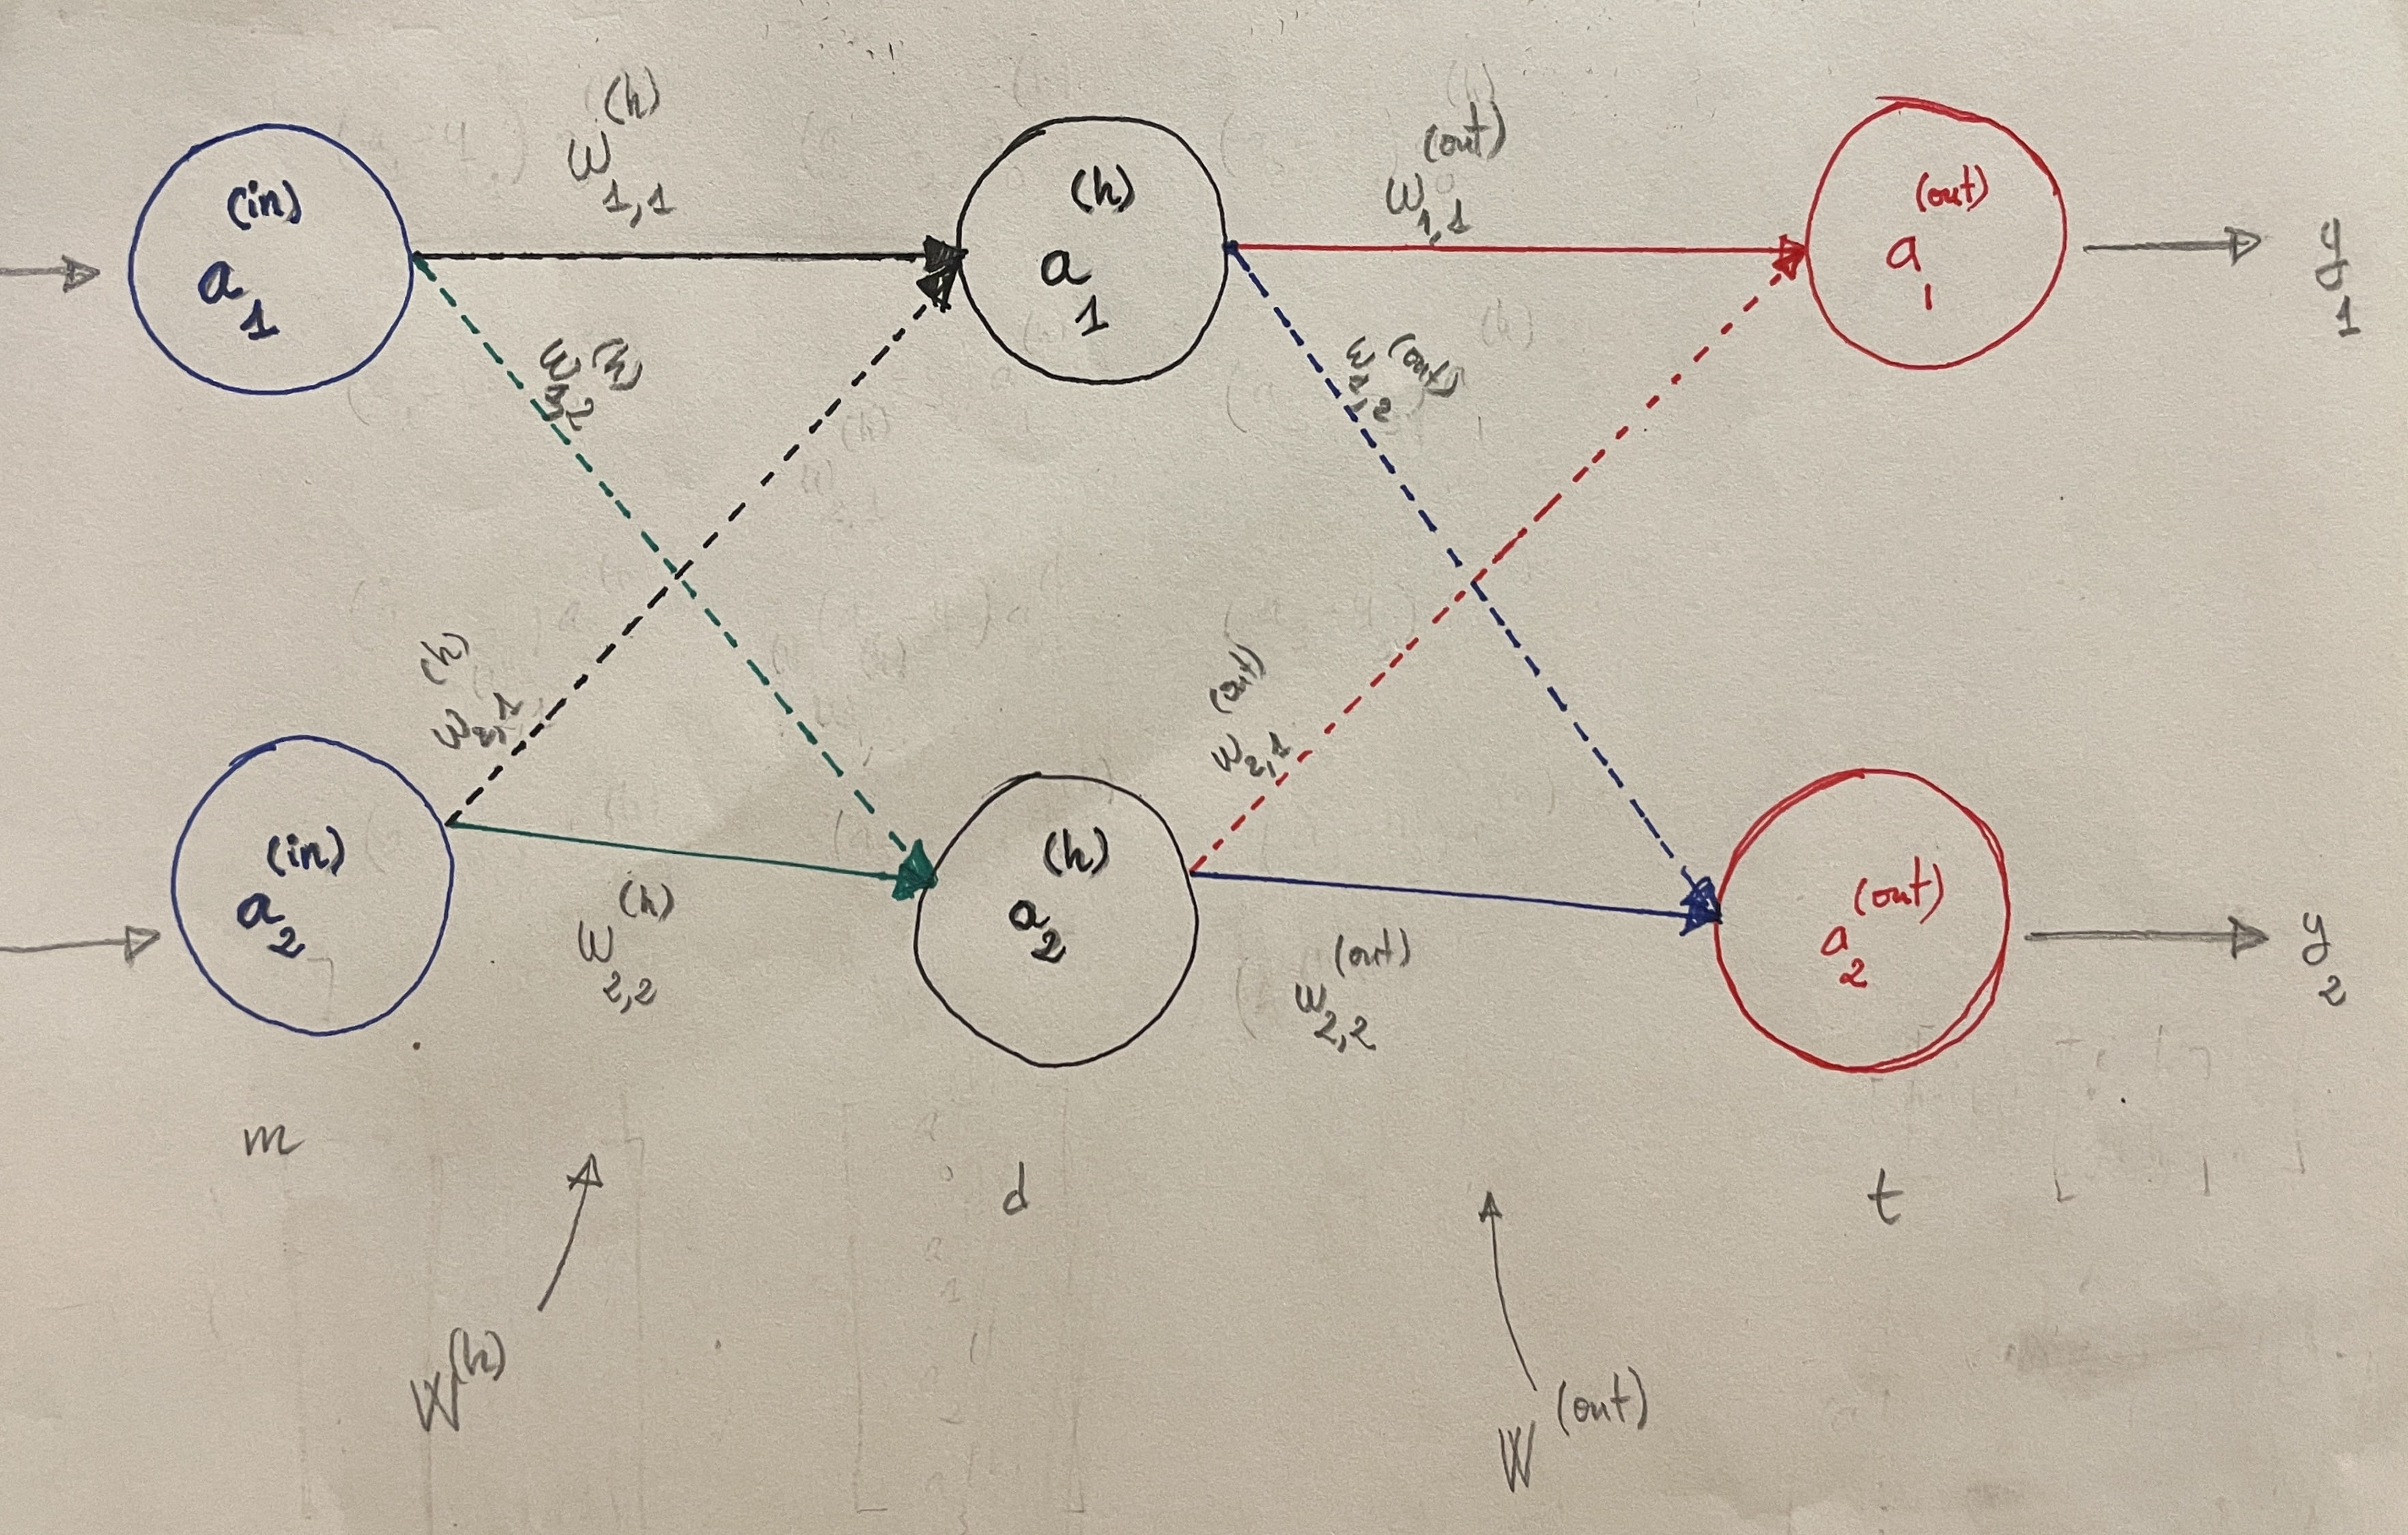
\includegraphics[width = 16cm, height = 9cm]{2-2-2-mlp.jpg}
\end{center}

\vspace{5mm} %5mm vertical space

We'll ignore biase units in the input and hidden layers, and 
consider only ONE training example for simplicity purposes.

\vspace{5mm} %5mm vertical space

Since one training example is considered and the network has
two output units, then  $n = 1$ and $t = 2$. So, the loss 
function becomes like this:

\[J(w) = -\sum\nolimits_{j=1}^{t} y_j^{[1]} ln(a_j^{[1]}) + (1 - y_j^{[1]})ln(1 - a_j^{[1]})\]

\vspace{5mm} %5mm vertical space

The journey of a SINGLE training example from the input layer to
the output layer of our network goes like this:

\vspace{5mm} %5mm vertical space

\pagebreak
\[[a_1^{(in)}, a_2^{(in)}]\]
\[\downarrow\]
\[W^{(h)}\]
\[\downarrow\]                  
\[[z_1^{(h)}, z_2^{(h)}]\]
\[\downarrow\]
\[\phi(\bullet)\]
\[\downarrow\]
\[[a_1^{(h)}, a_2^{(h)}]\]
\[\downarrow\]
\[W^{(out)}\]
\[\downarrow\]                  
\[[z_1^{(out)}, z_2^{(out)}]\]
\[\downarrow\]
\[\phi(\bullet)\]
\[\downarrow\]
\[[a_1^{(out)}, a_2^{(out)}]\]
\[\downarrow\]
\[[y_1, y_2]\]
\pagebreak

Now, let's compute the derivative of each  weights in the
$W^{(out)}$ matrix. To help myself, I drew the following
tree diagram to see how the variables in $J(W)$ relate to 
the weights in $W^{(out)}$:

\vspace{5mm} %5mm vertical space

\begin{figure}[h!]
    \centering
    \begin{forest}
        for tree={
            l sep=30pt,
            parent anchor=south,
            align=center
        }
            [$J(W)$
            [$y_1$]
            [$a_1^{(out)}$
                [$z_1^{(out)}$
                    [$w_{1,1}^{(out)}$]
                    [$w_{2,1}^{(out)}$]
                ]
            ]
            [$y_2$]
            [$a_2^{(out)}$
                [$z_2^{(out)}$
                    [$w_{1,2}^{(out)}$]
                    [$w_{2,2}^{(out)}$]
                ]
            ]
            ]
    \end{forest}
\end{figure}

Our MLP has two outputs. If you look at $J(W)$ expression 
closely, we compute the cost for each output, then add the results
together. And that's how we get the cost for the current training
example. With that in mind, we can now compute the partial
derivatives:

\vspace{5mm} %5mm vertical space

\[
    \frac{\partial J(W)}{\partial w_{1,1}^{(out)}} = 
    \frac{\partial J(W)}{\partial a_{1}^{(out)}} \times
    \frac{\partial a_{1}^{(out)}}{\partial z_{1}^{(out)}} \times
    \frac{\partial z_{1}^{(out)}}{\partial w_{1,1}^{(out)}}
\]

\[
    \frac{\partial J(W)}{\partial w_{2,1}^{(out)}} = 
    \frac{\partial J(W)}{\partial a_{1}^{(out)}} \times
    \frac{\partial a_{1}^{(out)}}{\partial z_{1}^{(out)}} \times
    \frac{\partial z_{1}^{(out)}}{\partial w_{2,1}^{(out)}}
\]

\[
    \frac{\partial J(W)}{\partial w_{1,2}^{(out)}} = 
    \frac{\partial J(W)}{\partial a_{2}^{(out)}} \times
    \frac{\partial a_{2}^{(out)}}{\partial z_{2}^{(out)}} \times
    \frac{\partial z_{2}^{(out)}}{\partial w_{1,2}^{(out)}}
\]

\[
    \frac{\partial J(W)}{\partial w_{2,2}^{(out)}} = 
    \frac{\partial J(W)}{\partial a_{2}^{(out)}} \times
    \frac{\partial a_{2}^{(out)}}{\partial z_{2}^{(out)}} \times
    \frac{\partial z_{2}^{(out)}}{\partial w_{2,2}^{(out)}}
\]

\vspace{5mm} %5mm vertical space

Notice, the following expressions are common in the first two and
last two equations. Let's evaluate them:

\[
    \frac{\partial J(W)}{\partial a_{1}^{(out)}} \times
    \frac{\partial a_{1}^{(out)}}{\partial z_{1}^{(out)}} = 
    (a_{1}^{(out)} - y_1) = \delta_1^{(out)}
\]

\[
    \frac{\partial J(W)}{\partial a_{2}^{(out)}} \times
    \frac{\partial a_{2}^{(out)}}{\partial z_{2}^{(out)}} = 
    (a_{2}^{(out)} - y_2) = \delta_2^{(out)}
\]

\vspace{5mm} %5mm vertical space

$(a_{1}^{(out)} - y_1)$ and $(a_{2}^{(out)} - y_2)$ are the 
``\textbf{error}" terms in the output layer. Since our MLP
has two outputs, we have two ``error" terms as well. We use 
``$\delta$" to denote that ``error". $\delta_1^{(out)}$ for 
instance, is the error in the first activation unit in the 
output layer.

\vspace{5mm} %5mm vertical space

With this new knowledge, we can re-write the partial derivatives:

\[
    \frac{\partial J(W)}{\partial w_{1,1}^{(out)}} =
    \delta_1^{(out)} a_1^{(h)}
\]

\[
    \frac{\partial J(W)}{\partial w_{2,1}^{(out)}} =
    \delta_1^{(out)} a_2^{(h)}
\]

\[
    \frac{\partial J(W)}{\partial w_{1,2}^{(out)}} =
    \delta_2^{(out)} a_1^{(h)}
\]

\[
    \frac{\partial J(W)}{\partial w_{2,2}^{(out)}} =
    \delta_2^{(out)} a_2^{(h)}
\]

From the above, I can now introduce the $\delta^{(out)}$ matrix.
It is a $n \times t$ matrix; where $n$ is the number of training
examples and $t$ the number of activation units in the output layer.
Since we are dealing with \underline{ONE} example and our MLP 
has \underline{2} outputs, so the $\delta^{(out)}$ matrix is of the 
shape $(1 \times 2)$, and looks like this:

\[
    \delta^{(out)} = [\delta_1^{(out)}, \delta_2^{(out)}] =
    [(a_{1}^{(out)} - y_1), (a_{2}^{(out)} - y_2)]
\]

\vspace{5mm} %5mm vertical space

Also, remember the $A^{(h)}$ matrix, obtained after training
examples are forward propagated from the input to the hidden layer.
Since we have \underline{ONE} training example and \underline{2}
units in the hidden layer. So $A^{(h)}$, is also of the shape
$(1 \times 2)$, and looks like this:

\[
    A^{(h)} = [a_1^{[1]}, a_2^{[1]}]
\]



\section{With a general $m-d-t$ MLP}
\end{document}